% !TEX root = ./Basilisk-rwMotorTorque-20190320.tex

\begin{figure}[htb]
	\centerline{
	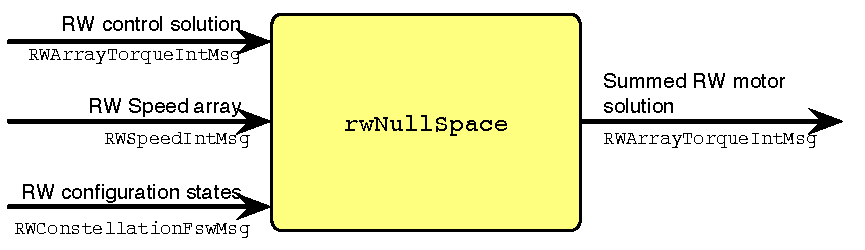
\includegraphics[]{Figures/moduleImg}
	}
	\caption{Illustration of Module Input and Output Messages}
	\label{fig:moduleImg}
\end{figure}


\section{Model Description}

\subsection{Module Input and Output Behavior}
As illustrated in Figure~\ref{fig:moduleImg}, this module takes an attitude control torque $\leftexp{B}{\bm L_{r}}$ and maps the vector onto the specific control axes, $\hat{\bm c}_{i}$.  This allows only a subset of $\leftexp{B}{\bm L_{r}}$ to be implemented with the Reaction Wheels (RWs).  The next step is to map reduced control torque onto  the available RW spin axes,$\hat{\bm g}_{s_j}$. The module accounts for the availability of the reaction wheels in the case that not all wheels are functioning appropriately or are undergoing independent analysis.  

Assume in this documentation that the number of available RWs is $m$, while the number of desired control axes $\hat{\bm c}_{i}$ is $n$.  The number of installed RWs is $N$.

The commanded torque message is a required input message and is read in every time step.  The RW configuration message is also required, but only read in during reset.  If the RW spin axes $\hat{\bm b}_{s_{i}}$ change then reset() must be called again.  The RW availability message is optional.  If the availability message is not used, then all installed RWs are assumed to be available.  The output message is always the array of RW motor torques.  



\subsection{Torque Mapping}
The {\tt rwMotorTorque} module receives a desired attitude control torque in the body frame $\leftexp{B}{\bm L}_r$.  This torque is the net control torque that should be applied to the spacecraft. Let $\hat{\bm g}_{s_{i}}$ be the individual RW spin axis, while $\bm u_{s}$ is the $m$-dimensional array of motor torques.  The $3\times m$ projection matrix $[G_{s}]$ then maps the control torque on motor torques using
\begin{equation}
	\label{eq:rwtm1}
	[G_{s}] \bm u_{s} = (-\leftexp{B}{\bm L}_r)
\end{equation}
The project matrix is defined as
\begin{equation}
	\label{eq:rwtm2}
	[G_{s}] = \begin{bmatrix}
		\hat{\bm g}_{s_{1}} & \cdots & \hat{\bm g}_{s_{m}}
	\end{bmatrix}
\end{equation}
Note that here $\bm u_{s}$ is the array of available motor torques.  The installed set of RWs could be larger than $m$.  

The projection matrix to map a vector in the body frame $\cal B$ onto the set of control axes $\hat{\bm c}_{i}$ is given by
\begin{equation}
	\label{eq:rwtm3}
	[CB] = \begin{bmatrix}
		\leftexp{B}{\hat{\bm c}}_{1}^{T}
		\\
		\vdots \\
		\leftexp{B}{\hat{\bm c}}_{n}^{T}
	\end{bmatrix}
\end{equation}
where $n \le 3$.  

To map the requested torque onto the control axes, Eq.~\eqref{eq:rwtm1} is pre-multifplied by $[CB]$ to yield
\begin{equation}
	\label{eq:rwtm4}
	[CB][G_{s}] \bm u_{s} = [CG_{s}] \bm u_{s} = [CB](-\leftexp{B}{\bm L}_r) = \leftexp{C}{\bm L}_{r}
\end{equation}
Note that $[CG_{s}]$ is a $n\times m$ matrix.  

The module assumes that $m\ge n$ such that there are enough RWs available to implement $ \leftexp{C}{\bm L}_{r}$.  If not, then the output motor torques are set to zero with $\bm u_{s} = \bm 0$.  

To invert Eq.~\eqref{eq:rwtm4} a minimum norm solution is used yielding: 
\begin{equation}
 \bm u_{s}  = [CG]^T \left([CG][CG]^T\right)^{-1}\  \leftexp{C}{\bm L}_{r}
\end{equation}
The final step is to map the array of available motor torques $\bm u_{s}$ onto the output array of installed RW motor torques.  


\subsection{RW Availability} 
If the input message name {\tt rwAvailInMsgName} is defined, then the RW availability message is read in. The torque mapping is only used for RW's whose availability setting is {\tt AVAILABLE}.  If it is {\tt UNAVAILABLE} then that RW output torque is set to zero.  

